\newpage
\section{Beschrijving van de Data.}
\label{sec:meth}

De data betreffende de Tweede Kamerverkiezingen van 2012 is een verzameling van open databestanden en databestanden verkregen van onderzoeksbureau IPSOS Nederland \citeyearpar{IPSOS}.
Ten doeleinde van dit onderzoek zijn verschillende dataset met elkaar gecombineerd om zodoende te pogen antwoorden te krijgen op de voor dit onderzoek opgestelde onderzoeksvragen. Met name voor de onderzoeksvraag betreffende het theoretisch maximum van vertegenwoordiging van bepaalde Nederlandse bevolkingsgroepen, is er data verzameld en zijn datasets met elkaar gecombineerd. De bevolkingsgroepen zijn: vrouwen, allochtonen, ouderen (met stemrecht en een leeftijd van 50 jaar en ouder) en provincialen (personen met stemrecht die buiten de Randstad-gemeenten wonen). Naast dataset die specifiek betrekking hebben tot één van de bevolkingsgroepen, zijn er ook algemene dataset gebruikt die op vrijwel alle bevolkingsgroepen van toepassing zijn. Allereerst volgt een beschrijving van de algemene datasets. Vervolgens worden per bevolkingsgroep de datasets beschreven.

\subsection*{Algemene Datasets.}
Wat de algemene data betreft gaat het hier om data die niet specifiek op één bevolkingsgroep betrekking had maar op meerdere bevolkingsgroepen. Deze dataset zijn: \\


\newcolumntype{L}{@{}>{\bfseries}p{13em}<{}}% Item label
\newcolumntype{I}{X@{}}% Item contents
\noindent\begin{tabularx}{\textwidth}{LI}
Landelijke peiling:  & Landelijke peiling aan de vooravond van de verkiezingen \citep{IPSOS}. In Figuur \ref{fig:pzL} is een grafiek te zien met de zetelverdeling  op basis van de peiling (licht gekleurde staven). \\
  \\
Kandidatenlijsten: & De kandidatenlijsten van de partijen die volgens de peiling kans maken op een zetel \citep{Kiesraad_kandidatenlijsten}. We gaan hierbij vanuit dat partijen die volgens de peiling geen zetel zouden gaan ontvangen ook bij de einduitslag geen zetel hebben ontvangen. In het geval van de Tweede Kamerverkiezingen van 2012 was dit ook daadwerkelijk het geval. Op de kandidatenlijsten stonden, naast de namen van de kandidaten, ook de plaats op de kandidatenlijst, de woonplaatsen en het geslacht van de kandidaten. In het geval van de PVDA en de SP moet genoteerd worden dat deze partijen bij de Tweede Kamerverkiezingen van 2012 gebruik hebben gemaakt van artikel H2 van de kieswet \citeyearpar{kieswetje}. Artikel H2 in de kieswet stelt dat partijen het recht hebben de laatste vijf kandidaten per kieskring te laten vari\"{e}ren. Voor dit onderzoek is besloten om de laatste vijf vari\"{e}rende kandidaten van de PVDA en de SP niet mee te nemen in het onderzoek. \\
\\
Offici\"{e}le verkiezingseinduitslag: & De officiële verkiezingseinduitslag van de Tweede Kamerverkiezingen van 12 september 2012 \citep{Kiesraad_databank}. De officiële verkiezingseinduitslag had ook het precieze aantal stemmen op een partij en op een kandidaat.  In Figuur \ref{fig:pzL} is een grafiek te zien met de zetelverdeling  op basis van de einduitslag (donker gekleurde staven).  \\
\\  
\end{tabularx}

\newcolumntype{L}{@{}>{\bfseries}p{13em}<{}}% Item label
\newcolumntype{I}{X@{}}% Item contents
\noindent\begin{tabularx}{\textwidth}{LI}
Gekozen kandidaten:  & De gekozen kandidaten na bekendmaking van de verkiezingseinduitslag van de Tweede Kamerverkiezingen van 12 september 2012 \citep{Kiesraad_uitslag}. Hierin zijn opgenomen: de namen van de gekozen kandidaten, de woonplaatsen van deze kandidaten en het aantal stemmen dat een kandidaat had ontvangen. \\
  \\
\end{tabularx}

\begin{figure}[H]
\centering
	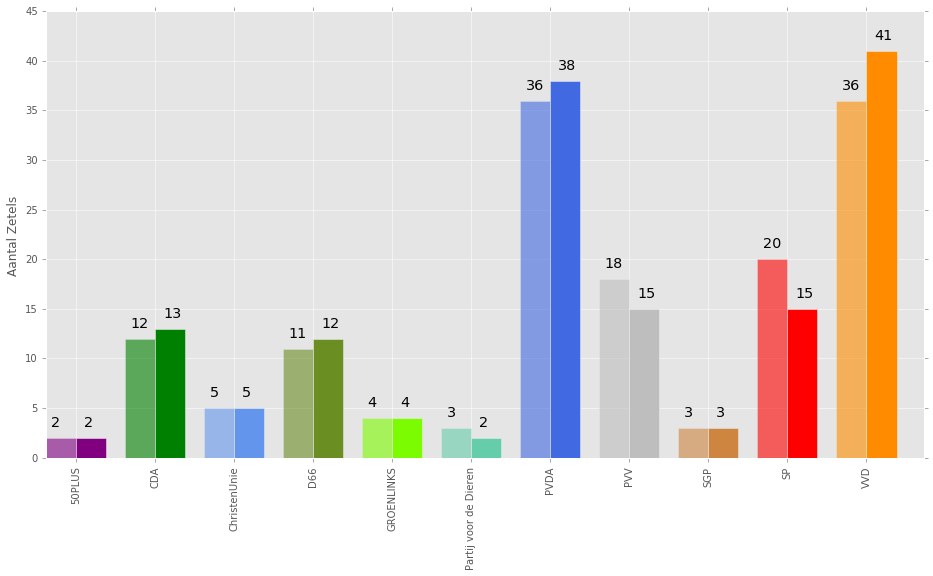
\includegraphics[width=\linewidth]{peiling_zetels_landelijk.png}

			\caption{De zetelverdelingen (licht gekleurd) volgens de peiling van 11 september 2012 \citep{IPSOS} en volgens de offici\"{e}le einduitslag (donker gekleurd) van 12 september 2012 \citep{Kiesraad_databank}.}

\label{fig:pzL}
\end{figure}











\subsection{Datasets betreffende de Bevolkingsgroep Vrouwen.}
De datasets betreffende de bevolkingsgroep vrouwen zijn:\\




\newcolumntype{L}{@{}>{\bfseries}p{13em}<{}}% Item label
\newcolumntype{I}{X@{}}% Item contents
\noindent\begin{tabularx}{\textwidth}{LI}
Geslacht: & Het geslacht van de kandidaten op de kandidatenlijsten van de partijen \cite{Kiesraad_kandidatenlijsten}. In de grafiek in Figuur \ref{fig:mvKandidaten} is het aantal mannelijke en vrouwelijke kandidaten op de kandidatenlijsten van de partijen te zien. Het gaat hierbij om enkel om partijen die volgens de peiling zetels zouden gaan ontvangen.\\
\\
Man-vrouw stemmenverdeling: & Man-vrouw verdeling in percentage van het totaal aantal uitgebrachte stemmen op een partij op basis van de einduitslag \citep{IPSOS}. In Tabel \ref{table:tab2V} (zie Sectie \ref{sssec:vrouwen}) zijn de mannelijke een vrouwelijke stempercentages te zien. \\
\\  
\end{tabularx}

\newcolumntype{L}{@{}>{\bfseries}p{13em}<{}}% Item label
\newcolumntype{I}{X@{}}% Item contents
\noindent\begin{tabularx}{\textwidth}{LI}
Ontbrekende data:  & Vanwege het ontbreken van data betreffende een peiling onder vrouwelijke kiezers nemen we aan dat de landelijke peiling toereikend is voor de peiling onder vrouwelijke kiezers. Zodoende gebruiken we de dataset met daarin de landelijke peiling als dataset voor de peiling onder vrouwelijke kiezers. \\
  \\
\end{tabularx}
\begin{figure}[H]
\centering
	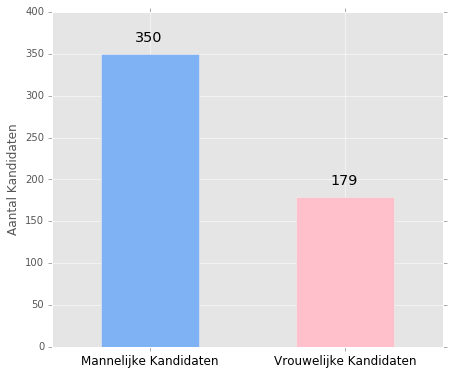
\includegraphics[width=0.42\linewidth]{mv_kandidaten.png}

			\caption{Het aantal mannelijke en vrouwelijk kandidaten op de kandidatenlijsten van de partijen die volgens de peiling zetels zouden gaan ontvangen.}

\label{fig:mvKandidaten}
\end{figure}



\subsection{Datasets betreffende de Bevolkingsgroep Allochtonen.}
De datasets betreffende de bevolkingsgroep allochtonen zijn:\\



\newcolumntype{L}{@{}>{\bfseries}p{13em}<{}}% Item label
\newcolumntype{I}{X@{}}% Item contents
\noindent\begin{tabularx}{\textwidth}{LI}
Peiling onder allochtonen: & Peiling onder westerse en niet-westerse allochtonen \citep{Opiniehuis}. In Tabel \ref{table:tab1A} (zie Sectie \ref{sssec:allochtonen}) is de verdeling volgens de peiling in percentages te zien.\\
\\
Bevolkingsaantallen: & Bevolkingsaantallen van westerse en niet-westerse allochtonen in Nederland \citep{CBS_allochtonen}. Op 1 september 2012 waren er 2.629.699 allochtonen boven de 18 jaar wonenden in Nederland. We gaan er voor deze bevolkingsgroep vanuit dat al deze personen stemgerechtigd waren tijdens de Tweede Kamerverkiezingen van 2012. \\
\\  
Stemgedrag:  & Stemgedrag van westerse en niet-westerse allochtonen \citep{CBS_stemgedrag}. Hierbij staat het aandeel allochtone stemmen op een partij tot verhouding met het totaal aantal uitgebrachte allochtone stemmen bij de Tweede Kamerverkiezingen. Dit noemen we het allochtone stempercentage. In de grafiek in Figuur \ref{table:tab2A} (zie Sectie \ref{sssec:allochtonen}) is op basis van de einduitslag de stemverdeling in percentages te zien.\\
 \\
\end{tabularx}

\newcolumntype{L}{@{}>{\bfseries}p{13em}<{}}% Item label
\newcolumntype{I}{X@{}}% Item contents
\noindent\begin{tabularx}{\textwidth}{LI}
Allochtone kandidaten: & De allochtone kandidaten op de kandidatenlijsten van de partijen. Hierbij moet genoteerd worden dat deze dataset deels zelf in elkaar is gezet. Onderzoeken van \citet{marinissen2013stemmen} en het Sio \citeyear{SIO} leverde al 33 allochtone kandidaten op. Echter waren deze kandidaten enkel van Marokkaanse, Turkse of Surinaamse afkomst. Voor de andere kandidaten is er ten behoeve van dit onderzoek gekeken of zij allochtoon zijn of niet. Hierbij zijn online bronnen geraadpleegd. In het geval dat twee of meerdere online bronnen aangaven dat een kandidaat als allochtoon geïdentificeerd kon worden, is de kandidaat toegevoegd aan de dataset. Het is daarom belangrijk te benadrukken dat er niet met 100\% zekerheid gesteld kan worden of een kandidaat allochtoon is of niet. Ter illustratie van het tot stand komen van de dataset nemen we Vera Bergkamp van D66 en Jenny Zerfowski van de PVV als voorbeelden.

\indent Vera Bergkamp heeft een, op het eerst gezicht, naam die niet snel aan een buitenlandse afkomst doet denken. Echter heeft Vera Bergkamp volgens \citet{allochtonie} en volgens \citet{zaman} een Marokaanse vader. Volgens de definitie van het CBS (zie VERWIJZING NAAR INTRODUCTIE) is Vera Bergkamp een allochtoon. Het volgende voorbeeld is Jenny Zerfowski van de PVV. Jenny Zerfowski heeft, in tegenstelling tot Vera Bergkamp, wel een buitenlands klinkende achternaam. Om haar enkel op basis van haar achternaam te identificeren als allochtoon zou niet toereikend zijn. Daarnaast is het de vraag of dit wel ethisch verantwoord is. Hoe dan ook is er ten behoeve van dit onderzoek gepoogd uit te zoeken of Jenny Zerfowski een allochtoon is. Volgens een artikel in de Volkskrant\citeyearpar{volkskrantjenny} en een interview met haar op \citet{binnenlandsbestuur} is Jenny Zerfowski in Duitsland geboren. Op deze wijze zijn er vijftig kandidaten als allochtoon geïdentificeerd. In de grafiek in Figuur \ref{fig:aaKandidaten} is het aantal autochtone en allochtone kandidaten te zien.\\
  \\
\end{tabularx}







\iffalse
\begin{figure}[H]
\centering
	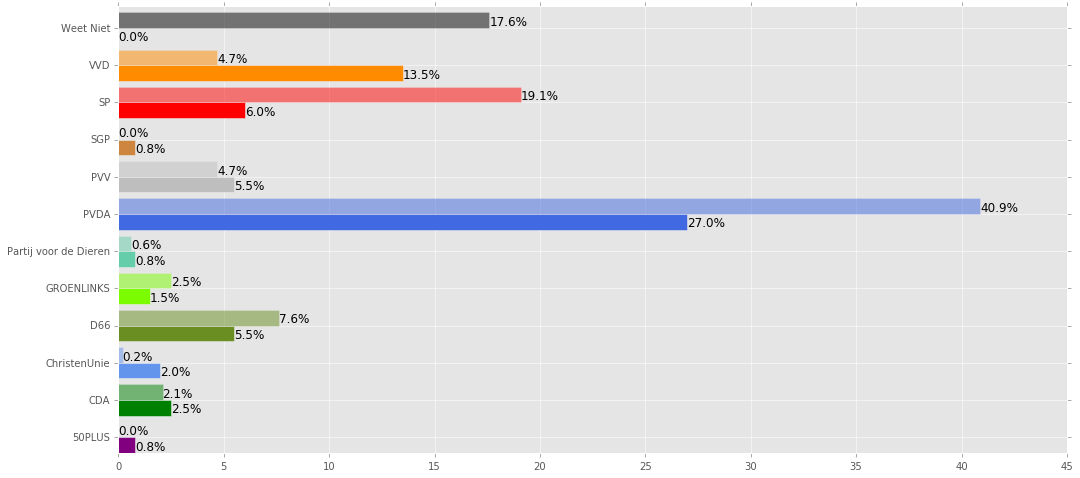
\includegraphics[width=\linewidth]{peiling_uitslag_percentages_allochtonen.png}

			\caption{De verdeling in procenten van allochtone stemmen op de partij volgens de peiling (licht gekleurd) en volgens de einduitslag (donker gekleurd).}

\label{fig:peil_uit_aa}
\end{figure}
\fi


\begin{figure}[H]
\centering
	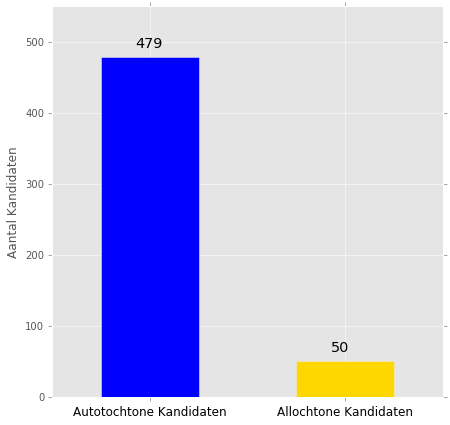
\includegraphics[width=0.42\linewidth]{aa_kandidaten.png}

			\caption{Het aantal autochtone en allochtone kandidaten op de kandidatenlijsten van de partijen die volgens de peiling zetels zouden gaan ontvangen.}

\label{fig:aaKandidaten}
\end{figure}


\subsection{Datasets betreffende de Bevolkingsgroep Ouderen.}
De datasets betreffende de bevolkingsgroep ouderen zijn:\\

\newcolumntype{L}{@{}>{\bfseries}p{13em}<{}}% Item label
\newcolumntype{I}{X@{}}% Item contents
\noindent\begin{tabularx}{\textwidth}{LI}
Bevolkingsaantallen: &Bevolkingsaantallen van ouderen \citep{CBS_allochtonen}. De bevolkingsaantallen van alle personen van vijftig jaar een ouder wonenden in Nederland op 1 september 2012. We nemen hierbij aan dat al deze personen stemgerechtigd zijn.   \\
\\  
Stemgedrag:  & Stemgedrag van ouderen \citep{CBS_stemgedrag}. Hierbij staat het aandeel oudere stemmen op een partij tot verhouding met het totaal aantal uitgebrachte oudere stemmen bij de Tweede Kamerverkiezingen. Dit noemen we het oudere stempercentage. \\
\\
Oudere kandidaten: & De oudere kandidaten op de kandidatenlijsten van de partijen \citep{allekandidaten}. Zie de grafiek in Figuur \ref{fig:jaKandidaten} voor het aantal kandidaten met een leeftijd van 50 jaar of jonger en het aantal oudere kandidaten op de kandidatenlijsten van de partijen die volgens de peiling zetels zouden gaan ontvangen. \\
  \\
Ontbrekende data: &  Vanwege het ontbreken van een peiling onder oudere kiezers nemen we aan de landelijk peiling toereikend is voor de peiling onder oudere kiezers. Zodoende gebruiken we de dataset met daarin de landelijk peiling als dataset voor de peiling onder oudere kiezers.\\
\\
 \end{tabularx}


\begin{figure}[H]
\centering
	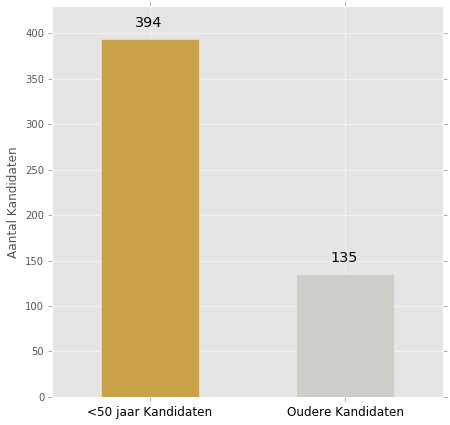
\includegraphics[width=0.42\linewidth]{ja_kandidaten.png}

			\caption{Het aantal kandidaten met een leeftijd van 50 jaar of jonger en het aantal oudere kandidaten op de kandidatenlijsten van de partijen die volgens de peiling zetels zouden gaan ontvangen.}

\label{fig:jaKandidaten}
\end{figure}


\newpage
\subsection{Datasets betreffende de Bevolkingsgroep Provincialen.}
De datasets betreffende de provincialen ouderen zijn:\\

\newcolumntype{L}{@{}>{\bfseries}p{13em}<{}}% Item label
\newcolumntype{I}{X@{}}% Item contents
\noindent\begin{tabularx}{\textwidth}{LI}
De Randstad-gemeenten: &  Er is in de literatuur geen eenduidige stelling over welke gemeenten precies tot de Randstad behoren. Daarmee is de exacte grens moeilijk vast te stellen \citep{nijmeijer2000randstad}. Daarom is de dataset met daarin de Randstad-gemeenten verkregen van Wikipedia \citeyearpar{randstad}. Hierbij is een kleine steekproef uitgevoerd om zodoende uit te vinden of een gemeente in de dataset daadwerkelijk tot de Randstad gerekend kan worden. Ter illustratie nemen we de gemeente Haarlem en vervolgens de gemeente Woerden als voorbeelden. 

\hspace*{1em} Voor de gemeente Haarlem is in twee verschillende online bronnen gevonden waarin er wordt gesteld dat de gemeente Haarlem in de Randstad ligt. Deze bronnen zijn de Trouw \citeyear{trouwhaarlem} en HP/De Tijd \citeyear{HPhaarlem}. Ook voor de gemeente Woerden is er in twee verschillende online bronnen gevonden dat er gesteld wordt dat de gemeente Woerden in de Randstad ligt. Deze bronnen zijn de gemeente Woerden \citeyear{gemeentewoerden} en Villa-Berlage \citeyear{villaberlage}. Op dezelfde wijze als voor deze twee gemeenten is gedaan, is dit ook voor de een aantal andere gemeenten in de dataset gedaan. Alle gemeenten die zijn meegenomen in de steekproef bevinden zich, volgens verschillende online bronnen, in de Randstad. Zodoende bleek uit de steekproef dat de dataset met daarin gemeenten in de Randstad een grote mate van betrouwbaarheid geniet. Via de Kiesraad \citeyearpar{Kiesraad_databank} is achterhaald hoeveel stemgerechtigden er in de Randstad-gemeenten woonden ten tijde van de Tweede Kamerverkiezingen van 2012.  \\
\\  
Aantal stemgerechtigden:  & Het aantal stemgerechtigde provincialen is tot stand gekomen door alle stemgerechtigden uit de Randstad-gemeenten \citep{randstad} af te trekken van het totaal aantal stemgerechtigden in Nederland ten tijde van de Tweede Kamerverkiezingen van 2012 \citep{Kiesraad_uitslag}.   \\
\\
Provinciale kandidaten: &  Voor het vaststellen of een kandidaat als provinciale kandidaat geïdentificeerd kan worden, is weer de dataset met daarin alle Randstad-gemeenten gebruikt \citep{randstad}. Door Randstad-gemeenten dataset te combineren met de kandidatenlijsten (hierin staan ook de woonplaatsen van de kandidaten) is er vastgesteld welke kandidaten wel en welke kandidaten er niet uit de Randstad-gemeenten afkomstig zijn.  Zie de grafiek in Figuur \ref{fig:rpKandidaten} voor het aantal Randstedelijke en provinciale kandidaten op de kandidatenlijsten van de partijen die volgens de peiling zetels zouden gaan ontvangen.\\
\\
 \end{tabularx}


\newcolumntype{L}{@{}>{\bfseries}p{13em}<{}}% Item label
\newcolumntype{I}{X@{}}% Item contents
\noindent\begin{tabularx}{\textwidth}{LI}
Ontbrekende data: &   Vanwege het ontbreken van data betreffende een peiling onder provinciale kiezers nemen we aan dat de landelijke peiling toereikend is voor de peiling onder provinciale kiezers. Zodoende gebruiken we de dataset met daarin de landelijke peiling als dataset voor de peiling onder provinciale kiezers.

\hspace*{1em} Naast het ontbreken van een peiling onder provincialen, ontbreekt ook de data betreffende het aandeel provinciale stemmen op een partij in verhouding tot het totaal aantal uitgebrachte provinciale stemmen bij de Tweede Kamerverkiezingen. Zodoende gebruiken we het landelijk stempercentage als stempercentage voor de provinciale stemmen.\\
\\
 \end{tabularx}



\begin{figure}[H]
\centering
	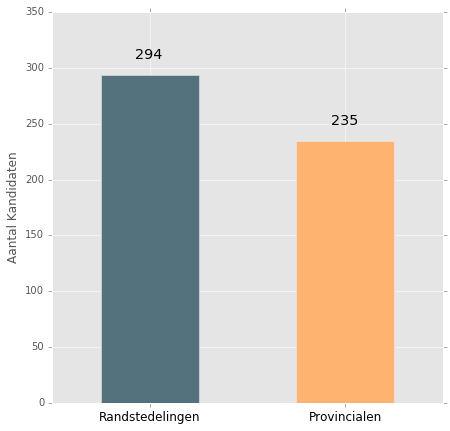
\includegraphics[width=0.42\linewidth]{rp_kandidaten.png}

			\caption{Het aantal Randstedelijke en provinciale kandidaten op de kandidatenlijsten van de partijen die volgens de peiling zetels zouden gaan ontvangen.}

\label{fig:rpKandidaten}
\end{figure}

















\iffalse

Data verzameling en beschrijving van de data jajaja

Hoe is de data verzameld, en hoe heb jij die data verkregen?


Wat staat er in de data? Niet alleen maar een technisch verhaal, maar ook inhoudelijk. DE lezer moet een goed idee krijgen over de technische inhoud en wat het betekent.

\newpage


\pagebreak
\subsection{Wat plotjes en tabelletjes}

Zie het IPython Notebook \url{PandasAndLatex.ipynb} voor de code om vanuit pandas een poltje op te slaan en een dataframe als tabel op te slaan. Het werkt ideaal! 

%De interrupties van Wilders staan beschreven in Figure~\ref{fig:wilders} en Tabel~~\ref{tab:Wilders}.


%\begin{figure}
%\begin{center}
%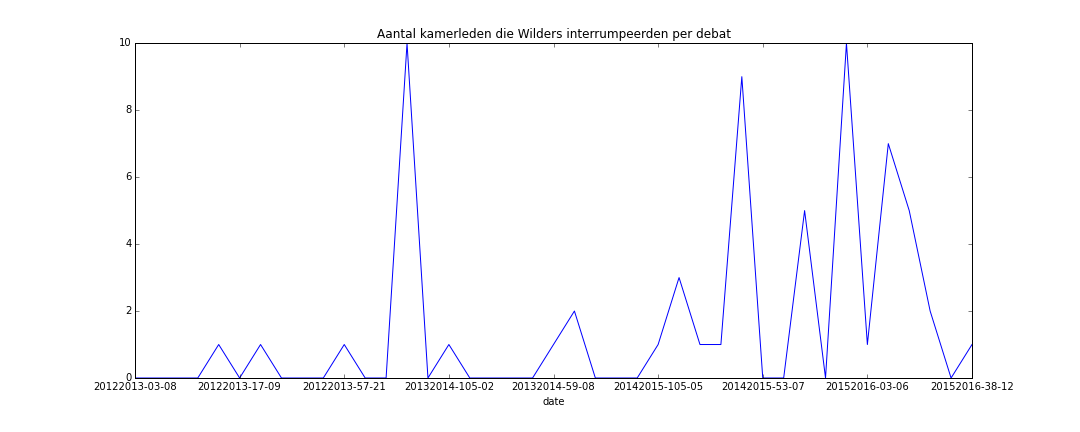
\includegraphics[width=\linewidth]{WildersPlot.png}
%\caption{\label{fig:wilders} Aantal interrupties van Wilders in de Tweede Kamer %door de tijd (periode 2012-2016).}
%\end{center}
%\end{figure}



\pagebreak


%\begin{table}[h]
%\begin{footnotesize}
%\begin{tabular}{lrl}
\toprule
{} &  indegree &                               interruptie\_volgorde \\
date            &           &                                                    \\
\midrule
20122013-03-08  &         0 &                                                    \\
20122013-07-16  &         0 &                                                    \\
20122013-100-03 &         0 &                                                    \\
20122013-100-06 &         0 &                                                    \\
20122013-17-06  &         1 &                         Pechtold-Pechtold-Pechtold \\
20122013-17-09  &         0 &                                                    \\
20122013-21-04  &         1 &                         Pechtold-Pechtold-Pechtold \\
20122013-22-08  &         0 &                                                    \\
20122013-32-06  &         0 &                                                    \\
20122013-48-23  &         0 &                                                    \\
20122013-57-21  &         1 &  Pechtold-Pechtold-Pechtold-Pechtold-Pechtold-P... \\
20122013-76-03  &         0 &                                                    \\
20122013-76-06  &         0 &                                                    \\
20132014-05-02  &        10 &  Roemer-Roemer-Van Haersma Buma-Van Haersma Bum... \\
20132014-06-04  &         0 &                                                    \\
20132014-105-02 &         1 &  Pechtold-Pechtold-Pechtold-Pechtold-Pechtold-P... \\
20132014-105-06 &         0 &                                                    \\
20132014-14-03  &         0 &                                                    \\
20132014-14-06  &         0 &                                                    \\
20132014-52-18  &         0 &                                                    \\
20132014-59-08  &         1 &                               Klaver-Klaver-Klaver \\
20142015-02-08  &         2 &  Pechtold-Pechtold-Pechtold-Pechtold-Pechtold-P... \\
20142015-03-06  &         0 &                                                    \\
20142015-09-09  &         0 &                                                    \\
20142015-100-05 &         0 &                                                    \\
20142015-105-05 &         1 &                                  Pechtold-Pechtold \\
20142015-111-04 &         3 &  Pechtold-Pechtold-Pechtold-Pechtold-Pechtold-P... \\
20142015-111-07 &         1 &                                  Pechtold-Pechtold \\
20142015-39-71  &         1 &                                  Pechtold-Pechtold \\
20142015-41-07  &         9 &  Samsom-Samsom-Pechtold-Pechtold-Pechtold-Kuzu-... \\
20142015-53-07  &         0 &                                                    \\
20142015-61-23  &         0 &                                                    \\
20142015-79-07  &         5 &  Klaver-Klaver-Klaver-Gesthuizen-Gesthuizen-Ges... \\
20142015-95-06  &         0 &                                                    \\
20152016-02-07  &        10 &  Pechtold-Pechtold-Pechtold-Pechtold-Slob-Slob-... \\
20152016-03-06  &         1 &       Pechtold-Pechtold-Pechtold-Pechtold-Pechtold \\
20152016-14-02  &         7 &  Klaver-Klaver-Roemer-Roemer-Roemer-Roemer-Sams... \\
20152016-14-05  &         5 &  Van Haersma Buma-Van Haersma Buma-Van Haersma ... \\
20152016-27-03  &         2 &  Segers-Segers-Segers-Segers-Kuzu-Kuzu-Kuzu-Kuz... \\
20152016-38-10  &         0 &                                                    \\
20152016-38-12  &         1 &                                        Klein-Klein \\
\bottomrule
\end{tabular}

%\end{footnotesize}
%\caption{\label{tab:Wilders} Door wie werd Wilders onderbroken en hoe vaak per debat.}
%\end{table}

%\begin{table}[h]
%	\begin{footnotesize}
%		\begin{tabular}{lrr}
\toprule
{} &  Aantal Stemmen Partij &  Aantal Stemmen Van Vrouwen \\
Partij                &                        &                             \\
\midrule
50PLUS                &                 123514 &                       61757 \\
CDA                   &                 741084 &                      370542 \\
ChristenUnie          &                 308785 &                      154392 \\
D66                   &                 679327 &                      339663 \\
GROENLINKS            &                 247028 &                      123514 \\
Partij v d Dieren &                 185271 &                       92635 \\
PVDA                  &                2223254 &                     1111627 \\
PVV                   &                1111627 &                      555813 \\
SGP                   &                 185271 &                       92635 \\
SP                    &                1235141 &                      617570 \\
VVD                   &                2223254 &                     1111627 \\
\bottomrule
\end{tabular}

%	\end{footnotesize}
%		\caption{\label{tab:Figuur1} Door wie werd Wilders onderbroken en hoe vaak per debat.}
%\end{table}

\pagebreak
\subsection{Methods}
Hoe je je vraag gaat beantwoorden.


Dit is de langste sectie van je scriptie. 

Als iets erg technisch wordt kan je een deel naar de Appendix verplaatsen. 

Probeer er een lopend verhaal van te maken.

Het is heel handig dit ook weer op te delen nav je deelvragen:

\subsubsection{RQ1}

\subsubsection{RQ2}
\fi
